% Options for packages loaded elsewhere
\PassOptionsToPackage{unicode}{hyperref}
\PassOptionsToPackage{hyphens}{url}
%
\documentclass[
  ignorenonframetext,
]{beamer}
\title{Workshop Pilot}
\subtitle{``How to work with data''\\
University of Urbino\\
PhD Program in Global Studies}
\author{Andrés Aguilera Castillo \and Luis Carlos Castillo}
\date{05 April 2022}

\usepackage{pgfpages}
\setbeamertemplate{caption}[numbered]
\setbeamertemplate{caption label separator}{: }
\setbeamercolor{caption name}{fg=normal text.fg}
\beamertemplatenavigationsymbolsempty
% Prevent slide breaks in the middle of a paragraph
\widowpenalties 1 10000
\raggedbottom
\setbeamertemplate{part page}{
  \centering
  \begin{beamercolorbox}[sep=16pt,center]{part title}
    \usebeamerfont{part title}\insertpart\par
  \end{beamercolorbox}
}
\setbeamertemplate{section page}{
  \centering
  \begin{beamercolorbox}[sep=12pt,center]{part title}
    \usebeamerfont{section title}\insertsection\par
  \end{beamercolorbox}
}
\setbeamertemplate{subsection page}{
  \centering
  \begin{beamercolorbox}[sep=8pt,center]{part title}
    \usebeamerfont{subsection title}\insertsubsection\par
  \end{beamercolorbox}
}
\AtBeginPart{
  \frame{\partpage}
}
\AtBeginSection{
  \ifbibliography
  \else
    \frame{\sectionpage}
  \fi
}
\AtBeginSubsection{
  \frame{\subsectionpage}
}
\usepackage{amsmath,amssymb}
\usepackage{lmodern}
\usepackage{iftex}
\ifPDFTeX
  \usepackage[T1]{fontenc}
  \usepackage[utf8]{inputenc}
  \usepackage{textcomp} % provide euro and other symbols
\else % if luatex or xetex
  \usepackage{unicode-math}
  \defaultfontfeatures{Scale=MatchLowercase}
  \defaultfontfeatures[\rmfamily]{Ligatures=TeX,Scale=1}
\fi
% Use upquote if available, for straight quotes in verbatim environments
\IfFileExists{upquote.sty}{\usepackage{upquote}}{}
\IfFileExists{microtype.sty}{% use microtype if available
  \usepackage[]{microtype}
  \UseMicrotypeSet[protrusion]{basicmath} % disable protrusion for tt fonts
}{}
\makeatletter
\@ifundefined{KOMAClassName}{% if non-KOMA class
  \IfFileExists{parskip.sty}{%
    \usepackage{parskip}
  }{% else
    \setlength{\parindent}{0pt}
    \setlength{\parskip}{6pt plus 2pt minus 1pt}}
}{% if KOMA class
  \KOMAoptions{parskip=half}}
\makeatother
\usepackage{xcolor}
\IfFileExists{xurl.sty}{\usepackage{xurl}}{} % add URL line breaks if available
\IfFileExists{bookmark.sty}{\usepackage{bookmark}}{\usepackage{hyperref}}
\hypersetup{
  pdftitle={Workshop Pilot},
  pdfauthor={Andrés Aguilera Castillo; Luis Carlos Castillo},
  hidelinks,
  pdfcreator={LaTeX via pandoc}}
\urlstyle{same} % disable monospaced font for URLs
\newif\ifbibliography
\setlength{\emergencystretch}{3em} % prevent overfull lines
\providecommand{\tightlist}{%
  \setlength{\itemsep}{0pt}\setlength{\parskip}{0pt}}
\setcounter{secnumdepth}{-\maxdimen} % remove section numbering
\ifLuaTeX
  \usepackage{selnolig}  % disable illegal ligatures
\fi

\begin{document}
\frame{\titlepage}

\begin{frame}{Double check for installation}
\protect\hypertarget{double-check-for-installation}{}
\begin{itemize}
\item
  Did you download and install Zotero / Mendeley / EndNote?

  --\textgreater{} Troubleshoot: Go to Workshop email click relevant
  link
\item
  Do you have an account in Web of Science?

  --\textgreater{} Troubleshoot: uniurb.it --\textgreater IRIS RICERCA
  --\textgreater{} Web of Science
\end{itemize}
\end{frame}

\begin{frame}{Computational Tools for Research}
\protect\hypertarget{computational-tools-for-research}{}
\begin{center}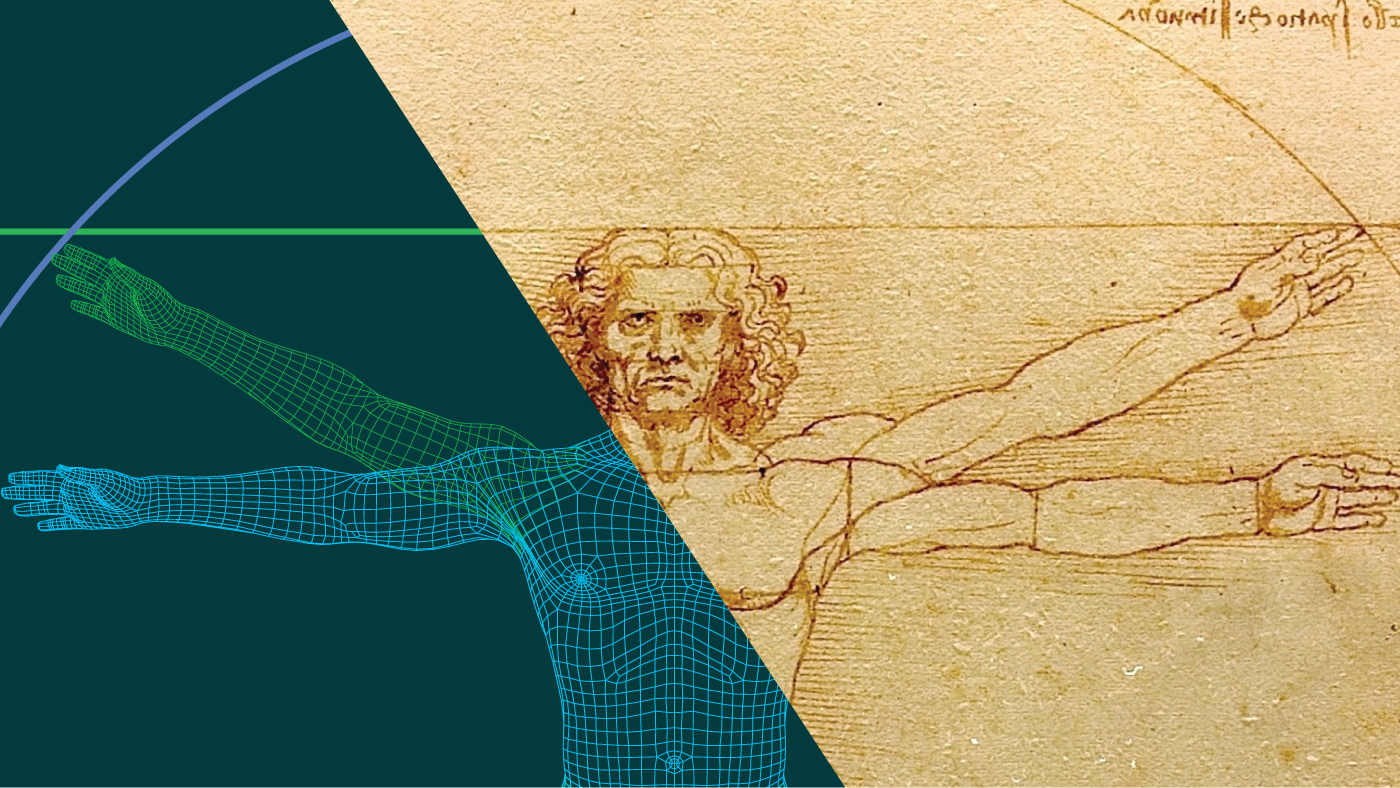
\includegraphics[width=0.75\linewidth]{/Users/lcastillot/Dropbox/Tesis/2021/Italy/Urbino/Data/Repos/workshop_uniurb/Images/unnamed} \end{center}
\end{frame}

\begin{frame}{Growth in scientific output and data available since 1980}
\protect\hypertarget{growth-in-scientific-output-and-data-available-since-1980}{}
Bornmann \& Mutz 2015

\begin{center}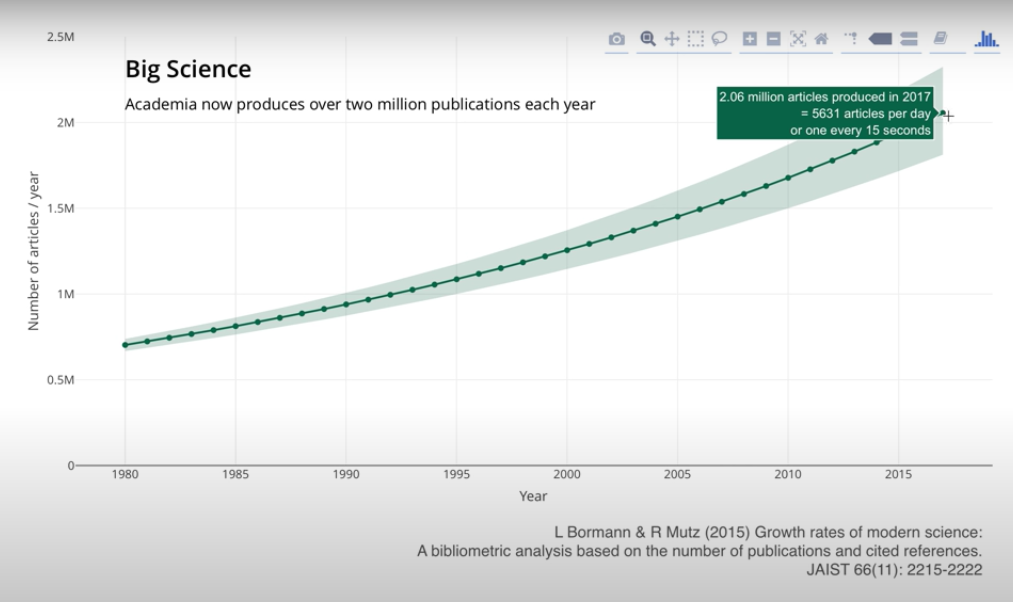
\includegraphics[width=0.75\linewidth]{/Users/lcastillot/Dropbox/Tesis/2021/Italy/Urbino/Data/Repos/workshop_uniurb/Images/Big_Science} \end{center}
\end{frame}

\begin{frame}{Replicability imperative}
\protect\hypertarget{replicability-imperative}{}
\begin{center}
\includegraphics[width=0.75\linewidth]{/Users/lcastillot/Dropbox/Tesis/2021/Italy/Urbino/Data/Repos/workshop_uniurb/Images/replicability} \end{center}
\end{frame}

\begin{frame}{New tools and Best practices}
\protect\hypertarget{new-tools-and-best-practices}{}
For both QL \& QT Better teamwork, allocation of tasks and effort
(Cloud)

\begin{center}
\includegraphics[width=0.75\linewidth]{/Users/lcastillot/Dropbox/Tesis/2021/Italy/Urbino/Data/Repos/workshop_uniurb/Images/ricerca_sviluppo} \end{center}
\end{frame}

\begin{frame}{Digital Transformation in Research}
\protect\hypertarget{digital-transformation-in-research}{}
\begin{center}
\includegraphics[width=0.75\linewidth]{/Users/lcastillot/Dropbox/Tesis/2021/Italy/Urbino/Data/Repos/workshop_uniurb/Images/teams_win} \end{center}
\end{frame}

\begin{frame}{PART 2}
\protect\hypertarget{part-2}{}
\begin{block}{Reference Management Systems}
\protect\hypertarget{reference-management-systems}{}
\end{block}
\end{frame}

\begin{frame}{Basic Workflow: Incoming to Reference Manager}
\protect\hypertarget{basic-workflow-incoming-to-reference-manager}{}
\begin{center}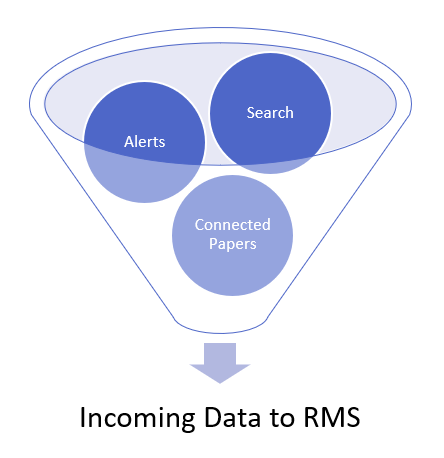
\includegraphics[width=0.55\linewidth]{/Users/lcastillot/Dropbox/Tesis/2021/Italy/Urbino/Data/Repos/workshop_uniurb/Images/Incoming} \end{center}
\end{frame}

\begin{frame}{Basic Workflow: Quality Control}
\protect\hypertarget{basic-workflow-quality-control}{}
\begin{center}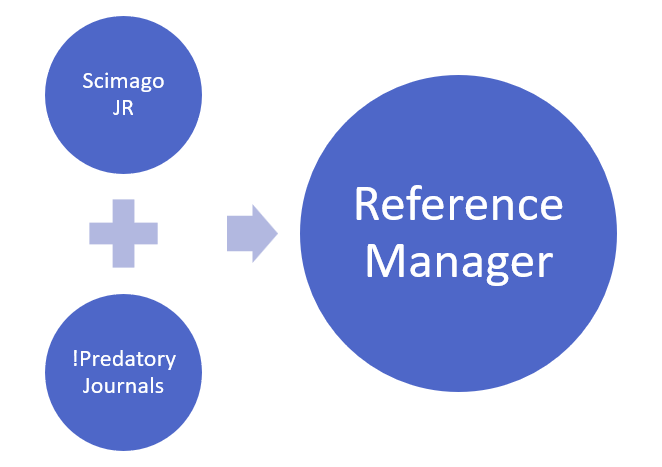
\includegraphics[width=0.5\linewidth]{/Users/lcastillot/Dropbox/Tesis/2021/Italy/Urbino/Data/Repos/workshop_uniurb/Images/quality_control} \end{center}
\end{frame}

\begin{frame}{Basic Workflow: Add to Reference Manager}
\protect\hypertarget{basic-workflow-add-to-reference-manager}{}
\begin{center}
\includegraphics[width=0.4\linewidth]{/Users/lcastillot/Dropbox/Tesis/2021/Italy/Urbino/Data/Repos/workshop_uniurb/Images/plugin} \end{center}
\end{frame}

\begin{frame}{Basic Workflow: Cite and Reference}
\protect\hypertarget{basic-workflow-cite-and-reference}{}
\begin{center}
\includegraphics[width=0.85\linewidth]{/Users/lcastillot/Dropbox/Tesis/2021/Italy/Urbino/Data/Repos/workshop_uniurb/Images/reference} \end{center}
\end{frame}

\begin{frame}{PART 3}
\protect\hypertarget{part-3}{}
\begin{block}{Web of Science Demonstration 🔑}
\protect\hypertarget{web-of-science-demonstration}{}
\end{block}

\begin{block}{How to search scientific papers 🗃️}
\protect\hypertarget{how-to-search-scientific-papers}{}
\end{block}

\begin{block}{How to create alerts 🔔}
\protect\hypertarget{how-to-create-alerts}{}
\end{block}
\end{frame}

\begin{frame}{Let's get started}
\protect\hypertarget{lets-get-started}{}
Go to uniurb.it -\textgreater{} IRIS RICERCA

Click WoS Create account
\end{frame}

\begin{frame}{Build better searches for systematic literature review}
\protect\hypertarget{build-better-searches-for-systematic-literature-review}{}
\end{frame}

\end{document}
